\documentclass[17pt,a4paper,landscape]{extarticle}
\usepackage[margin=2.35cm,top=0.12cm,left=1.05cm]{geometry}
\usepackage{amsmath}
\usepackage{amssymb}
\usepackage{tasks}
\usepackage{tikz}
\usepackage{xcolor}
\usepackage[sfdefault,lf]{FiraSans}
\renewcommand{\familydefault}{\sfdefault}
\setlength{\parindent}{0pt}
\pagestyle{empty}
\settasks{label=\textbf{\arabic*.}, label-width=2.2em, item-indent=2.95em, column-sep=2.1cm, after-item-skip=4.7em}
\renewcommand{\arraystretch}{1.15}
\everymath{\displaystyle}

\begin{document}
\sffamily
\boldmath

\boldmath

\boldmath

\boldmath

\boldmath

\boldmath

{\LARGE \textbf{Comparing box-and-whisker graphs - CSSI — Excellence}}
\begin{tasks}(3)
\task {Analyse the three box-and-whisker graphs using CSSI and write a comparative paragraph.\\[0.4em]
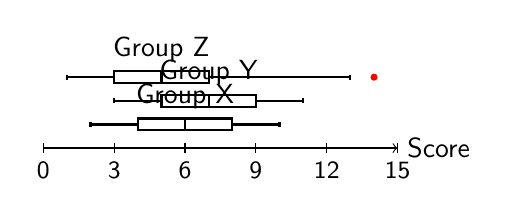
\begin{tikzpicture}[x=0.3cm,y=0.3cm,baseline=(current bounding box.center)]
  % axis
  \draw[->] (0,0) -- (15,0) node[right] {Score};
  \foreach \x in {0,3,6,9,12,15} \draw (\x,0.2) -- (\x,-0.2) node[below] {\small \x};
  % boxplot Group X
  \draw[thick] (2,1) -- (4,1);
  \draw[thick] (4,0.75) rectangle (8,1.25);
  \draw[thick] (6,0.75) -- (6,1.25);
  \draw[thick] (8,1) -- (10,1);
  \draw[thick] (2,0.9) -- (2,1.1);
  \draw[thick] (10,0.9) -- (10,1.1);
  \node[above] at (6,1.25) {Group X};
  % boxplot Group Y
  \draw[thick] (3,2) -- (5,2);
  \draw[thick] (5,1.75) rectangle (9,2.25);
  \draw[thick] (7,1.75) -- (7,2.25);
  \draw[thick] (9,2) -- (11,2);
  \draw[thick] (3,1.9) -- (3,2.1);
  \draw[thick] (11,1.9) -- (11,2.1);
  \node[above] at (7,2.25) {Group Y};
  % boxplot Group Z
  \draw[thick] (1,3) -- (3,3);
  \draw[thick] (3,2.75) rectangle (7,3.25);
  \draw[thick] (5,2.75) -- (5,3.25);
  \draw[thick] (7,3) -- (13,3);
  \draw[thick] (1,2.9) -- (1,3.1);
  \draw[thick] (13,2.9) -- (13,3.1);
  \fill[red] (14,3) circle (0.15);
  \node[above] at (5,3.25) {Group Z};
\end{tikzpicture}}
\task {Analyse the three box-and-whisker graphs using CSSI and write a comparative paragraph.\\[0.4em]
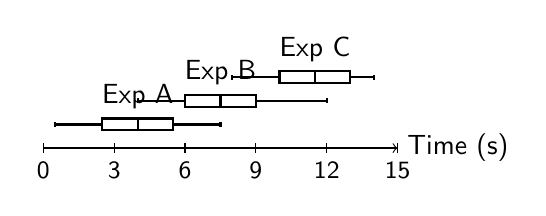
\begin{tikzpicture}[x=0.3cm,y=0.3cm,baseline=(current bounding box.center)]
  \draw[->] (0,0) -- (15,0) node[right] {Time (s)};
  \foreach \x in {0,3,6,9,12,15} \draw (\x,0.2) -- (\x,-0.2) node[below] {\small \x};
  % boxplot Experiment A
  \draw[thick] (0.5,1) -- (2.5,1);
  \draw[thick] (2.5,0.75) rectangle (5.5,1.25);
  \draw[thick] (4,0.75) -- (4,1.25);
  \draw[thick] (5.5,1) -- (7.5,1);
  \draw[thick] (0.5,0.9) -- (0.5,1.1);
  \draw[thick] (7.5,0.9) -- (7.5,1.1);
  \node[above] at (4,1.25) {Exp A};
  % boxplot Experiment B
  \draw[thick] (4,2) -- (6,2);
  \draw[thick] (6,1.75) rectangle (9,2.25);
  \draw[thick] (7.5,1.75) -- (7.5,2.25);
  \draw[thick] (9,2) -- (12,2);
  \draw[thick] (4,1.9) -- (4,2.1);
  \draw[thick] (12,1.9) -- (12,2.1);
  \node[above] at (7.5,2.25) {Exp B};
  % boxplot Experiment C
  \draw[thick] (8,3) -- (10,3);
  \draw[thick] (10,2.75) rectangle (13,3.25);
  \draw[thick] (11.5,2.75) -- (11.5,3.25);
  \draw[thick] (13,3) -- (14,3);
  \draw[thick] (8,2.9) -- (8,3.1);
  \draw[thick] (14,2.9) -- (14,3.1);
  \node[above] at (11.5,3.25) {Exp C};
\end{tikzpicture}}
\task {Analyse the three box-and-whisker graphs using CSSI and write a comparative paragraph.\\[0.4em]
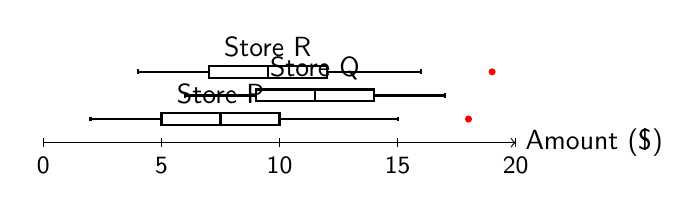
\begin{tikzpicture}[x=0.3cm,y=0.3cm,baseline=(current bounding box.center)]
  \draw[->] (0,0) -- (20,0) node[right] {Amount (\$)};
  \foreach \x in {0,5,10,15,20} \draw (\x,0.2) -- (\x,-0.2) node[below] {\small \x};
  % boxplot Store P
  \draw[thick] (2,1) -- (5,1);
  \draw[thick] (5,0.75) rectangle (10,1.25);
  \draw[thick] (7.5,0.75) -- (7.5,1.25);
  \draw[thick] (10,1) -- (15,1);
  \draw[thick] (2,0.9) -- (2,1.1);
  \draw[thick] (15,0.9) -- (15,1.1);
  \fill[red] (18,1) circle (0.15);
  \node[above] at (7.5,1.25) {Store P};
  % boxplot Store Q
  \draw[thick] (6,2) -- (9,2);
  \draw[thick] (9,1.75) rectangle (14,2.25);
  \draw[thick] (11.5,1.75) -- (11.5,2.25);
  \draw[thick] (14,2) -- (17,2);
  \draw[thick] (6,1.9) -- (6,2.1);
  \draw[thick] (17,1.9) -- (17,2.1);
  \node[above] at (11.5,2.25) {Store Q};
  % boxplot Store R
  \draw[thick] (4,3) -- (7,3);
  \draw[thick] (7,2.75) rectangle (12,3.25);
  \draw[thick] (9.5,2.75) -- (9.5,3.25);
  \draw[thick] (12,3) -- (16,3);
  \draw[thick] (4,2.9) -- (4,3.1);
  \draw[thick] (16,2.9) -- (16,3.1);
  \fill[red] (19,3) circle (0.15);
  \node[above] at (9.5,3.25) {Store R};
\end{tikzpicture}}
\task {For each set of three boxplots, write a full comparative analysis using CSSI.}
\task {Identify which group/experiment/store has the highest median and explain its significance.}
\task {Identify which group/experiment/store has the largest spread and explain its implications.}
\task {Identify any outliers and discuss their possible causes and effects on the data.}
\task {Discuss the shape of each distribution and what it suggests about the underlying data.}
\task {Compare the IQRs of the groups and discuss what this tells you about the variability within each group.}
\task {If you could only use one measure of centre and one measure of spread to compare these groups, which would you choose and why?}
\task {Suggest possible real-world contexts that could produce each set of boxplots.}
\task {Critique the use of boxplots for comparing these datasets. What are the limitations?}
\task {Propose a follow-up investigation based on the patterns you observed in the boxplots.}
\end{tasks}

\end{document}